\chapter{The Model}
This chapter explains the the paper "Convolutional neural network architecture for geometric matching\citep{Rocco17}" from Rocco, I. and Arandjelovi\'c, R. and Sivic, J. This paper gives a solution for the transformation between two images such as an affine transformation or thin-plate spline transformation, and estimating the parameters. This work gives the neural network model that we will build to try and solve our similar task involving the alignment of aerial images.

\section{Model}
In the geometric matching project\citep{Rocco17}, they propose a convolutional neural network architecture for geometric matching that includes three main components:
\begin{itemize}
\item CNN that mimics the standard steps of feature extraction.
\item the feature matching. 
\item simultaneous inlier detection and model parameter estimation.
\end{itemize}
  In a broad sense the process to align images with neural networks involves two approaches, a transfer learning approach to extract features, and a supervised learning approach to determine the affine transformation that will align features in paired images. Features can be extracted using a pre-trained neural network such as ResNet101\cite{dai2016r} or VGG-16\cite{simonyan2014very}. These are large networks originally designed to classify massive image datasets. We use the pre-trained model VGG 16 to do feature extraction. We crop off the last pooling layer of this network (before the ReLU activation) and perform L2 normalization. This is our transfer learning approach that uses the existing knowledge of images in the VGG 16 model. Our work here follows the work of Rocco\citep{Rocco17}. Feature regression (also known as finding the best alignment between the features of two images) is the part where supervised machine learning and a labelled dataset such as that described in Chapter 3 is required. The whole model is shown in Figure 4.1.

\begin{figure}
\centering
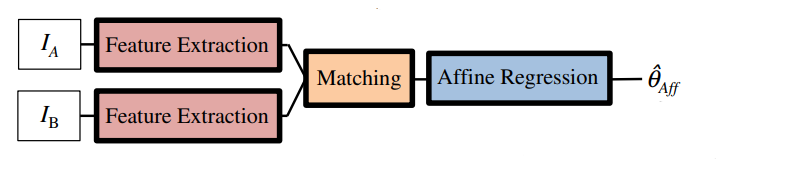
\includegraphics[width = 3.0in]{figs/cnn_model_aff}
\caption{CNN Model showing 3 steps in our process to arrive at $\theta$, which represents the transformation that can be applied to image $I_A$ to best align it with image $I_B$ (the inputs to the model).\cite{Rocco17}}
\end{figure}
\section{Input and output}
Refer to Figure 4.1, the input will be the two images that are passed into the model simultaneously (a source image and a target image). It should be noted that the images must have some overlap or commonalities, otherwise it makes no sense on how to align them. See Figure 4.2. The images go through the feature extraction CNN which is a pre-train neural network (VGG-16$pool4$) and return all the features that the network found in the input images. Note that Figure 4.2, only shows a few example features, simulated with red dots for clarity of understanding only.\\
  After feature extraction, we follow a L2-normalization to normalize all the features, and return the normalize features set for each image. After that we find the correlation between the normalized images. Feature correlation takes in two sets of the normalize features and returns a correlation tensor containing the correlation between each feature sets. We normalize the correlation in the same way that we normalize the extracted features.\\
  Estimating the parameters of the affine matrix is called feature regression, it is a CNN model that we train with our dataset, which takes in the normalized correlation sets and returns the affine matrix, denoted by $\theta$.
 
\begin{figure}
\centering
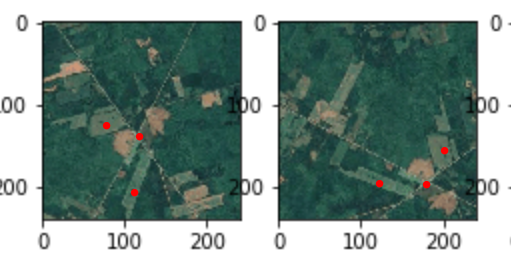
\includegraphics[width = 3.0in]{figs/data_example}
\caption{Two example images with red dots showing common points between the images. These images may be used as input to our model.}
\end{figure}
\section{Required label}
In order for the model to learn the affine transformation matrix, we need to pass the real matrix values to the model during the training phase, the affine transformation matrix  has six parameters, we put the matrix parameters in a csv file where each row of the file contains the following: A00, A01, tx, A10, A11, ty and their corresponding position in the affine transformation matrix given below:

$\begin{bmatrix}
A00& A01& tx \\
A10& A1& ty
\end{bmatrix}$\\
Rocco et al. \cite{Rocco18}, outline two ways to pass paired images and their corresponding affine transformation matrix into the model. One way is to only pass the source image path, and the parameter labels, which they call synth-dataset\cite{cnngeometric_pytorch}. The single image is altered to produce two images synthetically. The other way is passing the path to both a source and target image with labels and a bounding box giving the area in the image that is shared between the source and target. This is called a coupled-dataset \cite{cnngeometric_pytorch}, the coupled-dataset is what our work uses when we serve the training data to the model. 

\section{Learning}
In the paper\citep{Rocco17}, off which we base this project, the full model can be thought of as a pipeline (see Figure 4.3), the inputs to the pipeline are the source and target images. First step is to find features in the images, next we correlate the features and finally we determine the affine transformation aligning those features. This is done as part of a learning process, meaning the outputs are the raw values that make up the affine transformation matrix. Our goal is to adjust the neural network so that the outputs of the network match our labels, the ground truth affine transformations we already determined when we built the dataset.\\
  It should be noted that the goal of Rocco et al. \cite{Rocco17} differs from our own goal. See Figures 4.4,4.5 4.6 which show some of their results. The focus is on aligning certain aspects of an image, such as a car, or duck for instance.\\
  In our work we focus only on aerial photography. We assume that the photographs are taken from air planes with a camera pointing down and so viewing angles are less of a concern for us. We are only concerned with finding the affine transformation matrix between the two images. In some ways our task may be considered easier than Rocco et. al, because we do not concern ourselves with twists and deformations (such as deforming the duck in Figure 4.4, to match the target duck. However, our task may also be considered more difficult since we have images sometimes have a uniform appearance. For example an image with green fields. Finding features in such images could be quite challenging since the image looks the same in many parts.
\begin{figure}
\centering
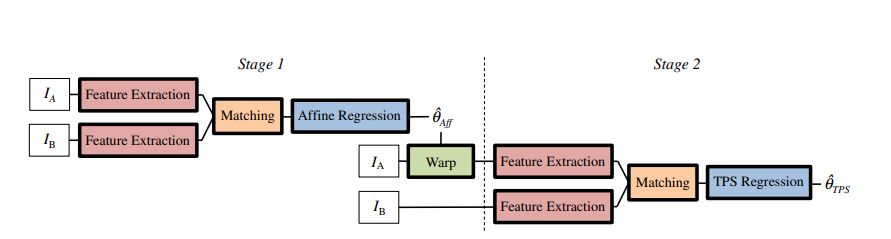
\includegraphics[width = 3.0in]{figs/full_arch}
\caption{The full model use by Rocco et, al.\cite{cnngeometric_pytorch}. Their full model was intended to warp and twist portions of an image for best alignment. We do not use the full model, as we assume aerial photographs to be roughly taken from the same relative position to the earth. In other words we assume the plane flies horizontal with a camera pointing down.}
\end{figure}
 The model learns how to apply affine transformation by finding the the key features in the source image and the target image, and find the transformations between the key features, apply each transformation to the source images and translate the images, finally, the model will apply affine transformation to the image, see Figure \ref{fig:4.3} shows how the source will translate corresponding on affine transformation. Also, the Figure \ref{fig: 4.4} marks the key points in the source image and the target image, also the translated images.\\ 
\begin{figure}
\centering
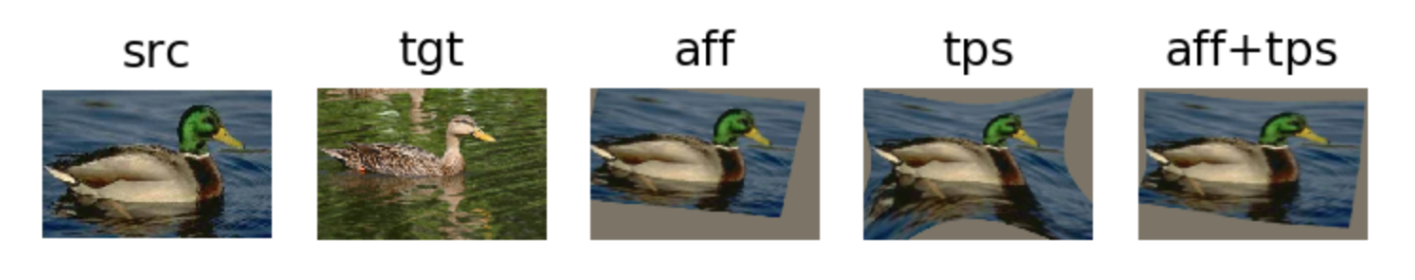
\includegraphics[width = 4.0in]{figs/aff_tps}
\caption{In the demonstration by Rocco et al\cite{Rocco17}, they show the alignment of two images containing similar ducks}
\end{figure}
The Figure 4.5 demonstrations of alignment between images that share characteristics. Note that a bounding box is used to single out the parts of the image that are in common. That the images are taking from "Qualitative results on the Tokyo Time Machine dataset\citep{Rocco18}".\\
\begin{figure}
\centering
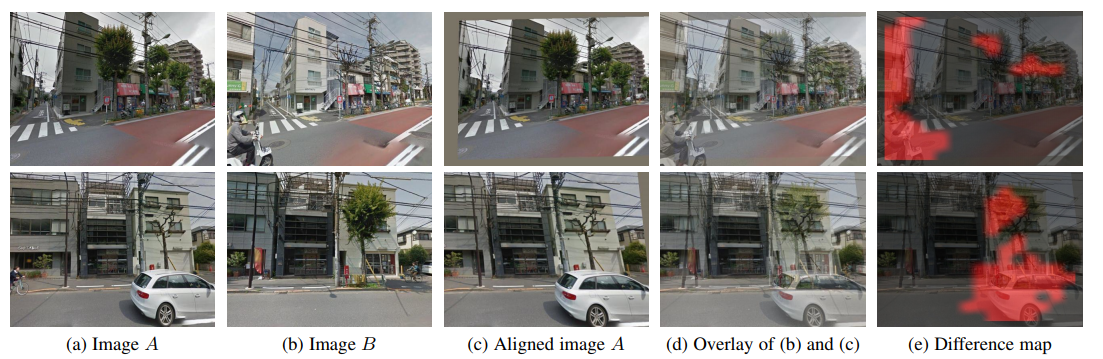
\includegraphics[width = 4.0in]{figs/overlap}
\caption{In the demonstration by Rocco et al\cite{Rocco18}, they show the finding the overlap between images}
\end{figure}
  The Figure 4.6 outline the boundary box that single out the key feature between images from the paper\citep{Rocco17}.
\begin{figure}
\centering
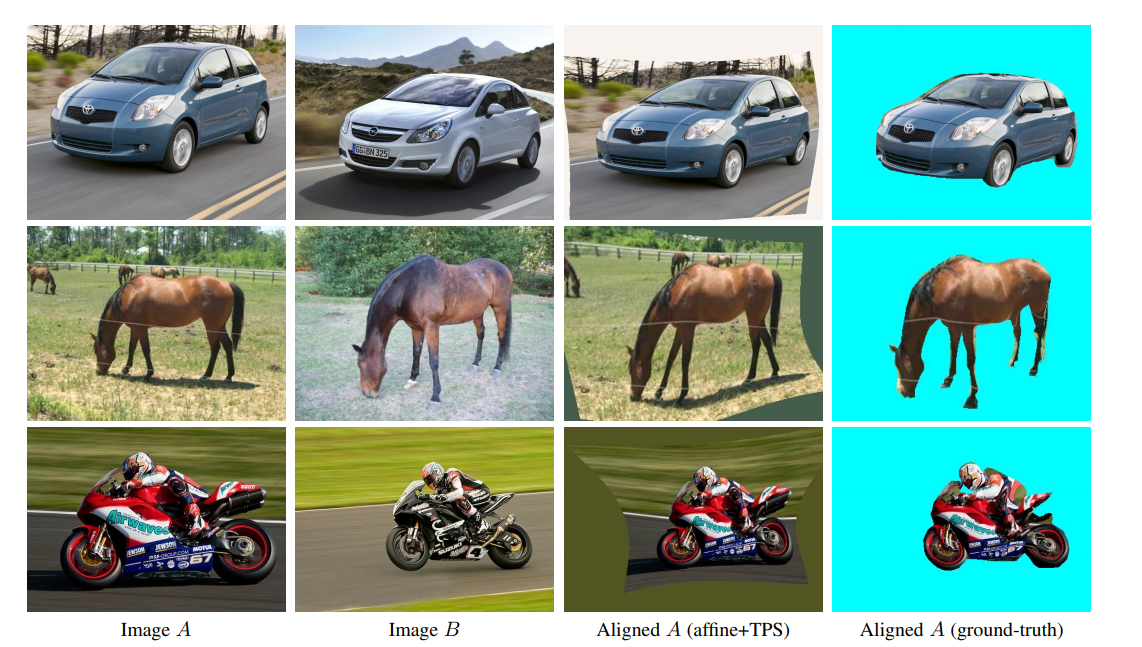
\includegraphics[width = 4.0in]{figs/bound_box}
\caption{In the demonstration by Rocco et al\cite{Rocco18}, they show the bounding box that single out the key feature between images}
\end{figure}
 

\begin{figure}
\centering
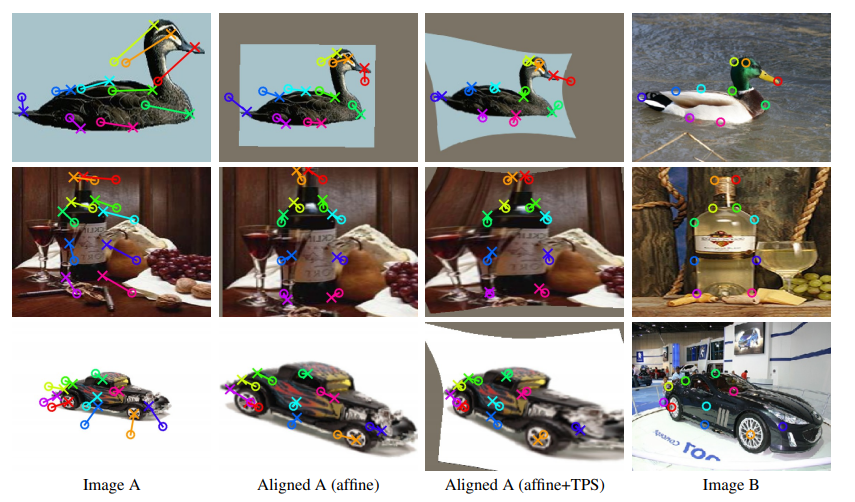
\includegraphics[width = 4.0in]{figs/keypoint_examples}
\caption{Model demo \cite{cnngeometric_pytorch}}
\end{figure}
  We are using the first part of the model and train it with our own aerial dataset and the model will learn how to find the affine transformation parameters between two aerial images. The model will concat with two neural network, the first part is a pre-trained neural network VGG16 that is used for feature extraction. The images each pass through the same network (our pretrained VGG 16 model) to extract image features. Recall the image features are computer distinguishable characteristics in the image, such as color changes, lines, corners, and various local pixel differences that respond to the convolutional filters. This follow by the layer matches those features, the matching layer use a correlation layer followed by normalization. First, all pairs of similarities
between descriptors are computed in the correlation layer. Secondly, similarity scores are processed and normalized such that ambiguous matches are strongly down-weighted\cite{Rocco17}.
The last part of the model is the regression network, which directly estimates parameters of the geometric transformation relating the two input images.\\
  As we mentioned previously a neural network requires a cost function to facilitate training. In other words a measure of how wrong the network is. For this task we use mean squared error \cite{mse}. Mean squared error gives a measure of the average squared difference between the estimated values and the ground truth value. In our case MSE is calculated between the individual values that make up the affine transformation matrix that the model produces and the individual values that make up the affine transformation matrix in our ground truth.\\
  There are other cost functions that may be used. For example in Rocco et, al. \cite{Rocco17} they also propose a cost function that applies the generated transformation to the source image and compares pixels in the newly generated image and the ground truth applied to the source image. We discuss our cost function in further details in the next chapter.
